\documentclass[tikz, footheight=2em]{beamer}
\usetheme[hideothersubsections]{Hannover}
\usepackage[T1]{fontenc}
\usepackage[utf8]{inputenc}
\usepackage{amssymb}
\usepackage{amsthm}
\usepackage{amsmath}
\usepackage{color,graphicx}
\usepackage{ulem}
\usepackage{gensymb}
\usepackage[]{tikz}
\usetikzlibrary{quotes,angles}
\usepackage{tikz}
\usetikzlibrary{arrows}
\usetikzlibrary{calc}
\usetikzlibrary{positioning}

\usecolortheme{dolphin}

\title{Projet avion mineure AVI}
\author{Damien Thoral, Gabriel Hondet, Benoit Viry}
\date{}

% ----------------------------------------------------------
% nuremotation des pages -----------------------------------
% ----------------------------------------------------------
\def\swidth{1.6cm}
\setbeamersize{sidebar width left=\swidth}
\setbeamertemplate{sidebar left}
{%
  {\usebeamerfont{title in sidebar}
    \vskip1.5em
    \usebeamercolor[fg]{title in sidebar}
    \insertshorttitle[width=\swidth,center,respectlinebreaks]\par
    \vskip1.25em
  }
  {
    \usebeamercolor[fg]{author in sidebar}
    \usebeamerfont{author in sidebar}
    \insertshortauthor[width=\swidth,center,respectlinebreaks]\par
    \vskip1.25em
  }
  \hbox to2cm{\hss\insertlogo\hss}
  \vskip1.25em
  \insertverticalnavigation{\swidth}
  \vfill
  \hbox to2cm{\hskip0.6cm\usebeamerfont{subsection in
      sidebar}\strut\usebeamercolor[fg]{subsection in
      sidebar}\insertframenumber /\inserttotalframenumber\hfill}
  \vskip3pt
}
% ----------------------------------------------------------


\begin{document}

\frame{\titlepage}

\AtBeginSection[]
{%
  \begin{frame}
    \frametitle{Plan}
    \tableofcontents[currentsection]
  \end{frame}
}
\section{Introduction et modèle avion}

\begin{frame}
    \frametitle{Objectifs} \pause{}
    \begin{center}
        Étude de la dynamique d'un avion pour l'implemenation d'un pilote
        automatique.
    \end{center} \pause{}
    Motivation:
    \begin{center}
        le pilote souhaite commander son avion avec des instructions de haut
        niveau, ie suivre une route, un axe avec la présence de vent, commander
        une altitude ou une vitesse.
    \end{center}
\end{frame}

% \subsection{Rappels}
\begin{frame}
    \frametitle{Rappel équations de la dynamique} \pause{}
    En assimilant l'avion à un point on a:
    \[
    \left \{
    \begin{array}{l}
        m\dot{V} = T - D - mg\sin \gamma \\
        mV\dot{\gamma} = L\cos \phi - mg \cos \gamma \\
        mV \cos (\gamma) \dot{\psi} = L \sin \phi \\
        \dot{\phi} = p
    \end{array}
    \right.
    \] \pause{}

    Facteurs de charges longitudinal et vertical:
    \[
    n_x = \frac{T - D}{mg} \qquad n_z = \frac{L}{mg}
    \] \pause{}
    \begin{center}
        \fbox{
        On commande l'avion à l'aide de \( nx \), \( nz \) et \( p \)
        }
    \end{center}
\end{frame}

% \subsection{Facteur de charge}
\begin{frame}
    \frametitle{\(n_z = \frac{L}{mg}\) pour un virage}\pause{}
    En palier: \(\gamma = 0\) et \(\dot{\gamma} = 0\) \pause{}

    Avec \[ mV\dot{\gamma} = L\cos \phi - mg \cos \gamma \]
    on a \[ L=\frac{mg}{\cos \phi}\] \pause{}
    D'où:\[ \boxed{n_z = \frac{1}{\cos \phi}}\]
\end{frame}

\begin{frame}
    \frametitle{Rayon de virage}\pause{}
    En palier: \(\gamma = 0\) et \(\dot{\gamma} = 0\) \pause{}

    \[ \sout{m}V\dot{\psi} = \sout{m}g\tan \phi \] \pause{}
    avec

    \begin{center}
        \begin{tabular}{ccc}
            \(V = R\dot{\psi}\) & \(\Longrightarrow \) &
            \(\frac{V^2}{R} = g \tan \phi \)
        \end{tabular}
    \end{center}\pause{}

    D'où le rayon de virage:
    \[ \boxed{R = \frac{V^2}{g\tan \phi}}\]
\end{frame}

% % \subsection{$n_z$ ressource}

\begin{frame}
    \frametitle{\(n_z = \frac{L}{mg}\) pour une ressource}\pause{}
    En ressource: \(\phi = 0\) et \(\dot{\phi} = 0\)\pause{}

    Avec \[ mV\dot{\gamma} = L\cos \phi - mg \cos \gamma \]
    on a:\[ L = m(V\dot{\gamma} + g \cos \gamma)\] \pause{}
    D'où:\[ \boxed{n_z = \frac{V\dot{\gamma}}{g} + \cos \gamma}\]
\end{frame}

% \subsection{Représentation d'état}
\section{Linéarisation du modèle}


\begin{frame}
    \frametitle{Representation d'états non-linéaire}\pause{}
    Notons:
    \[
    \left \{
    \begin{array}{l}
        \underline{x}(t) = {[V(t), \gamma (t), \psi (t), \phi (t)]}^{T}\\
        \underline{u}(t) = {[n_x(t), n_z(t), p(t)]}^{T}
    \end{array}
    \right.
    \]\pause{}
    \[
    \left[
    \begin{array}{c}
        \dot{V}(t)\\
        \dot{\gamma}(t)\\
        \dot{\psi}(t)\\
        \dot{\phi}(t)
    \end{array}
    \right]
    =
    \left[
    \begin{array}{c}
        T - D - mg \sin \gamma \\
        \frac{L\cos \phi - mg\cos \gamma}{mV} \\
        \frac{L\sin \phi}{mV\cos \gamma} \\
        p
    \end{array}
    \right]
    =
    \left[
    \begin{array}{c}
        g(n_x - \sin \gamma) \\
        \frac{g}{V}(n_z \cos \phi - \cos \gamma)\\
        g \frac{n_z \sin \phi}{V \cos \gamma} \\
        p
    \end{array}
    \right]
    \]\pause{}
    \[
    \underline{\dot{x}}(t)=f(\underline{x}(t),\underline{u}(t))
    \]
\end{frame}

% \subsection{Linéarisation}
\begin{frame}
    \frametitle{Point d'équilibre}\pause{}
    Trouvons un point d'équilibre
    \[
    \left \{
    \begin{array}{l}
        \underline{x_e} = {[V_e, \gamma_e, \psi_e, \phi_e]}^{T}\\
        \underline{u_e} = {[n_{xe}, n_{ze}, p_e]}^{T}
    \end{array}
    \right.
    \]
    Tel que:
    \[
    \underline{\dot{x}_e} = f(\underline{x_e}, \underline{u_e}) = 0
    \]\pause{}
    Soit:
    \[
    \left \{
    \begin{array}{l}
        g(n_{xe} - \sin \gamma_e) = 0\\
        \frac{g}{V_e}(n_{ze} \cos \phi_e - \cos \gamma_e) = 0\\
        g \frac{n_{ze} \sin \phi_e}{V_e \cos \gamma_e} = 0\\
        p_e = 0
    \end{array}
    \right.
    \]
\end{frame}

\begin{frame}
    \frametitle{Point d'équilibre}\pause{}
    D'où:
    \[
    \left \{
    \begin{array}{l}
        n_{xe} = \sin \gamma_e \\
        n_{ze} \cos \phi_e = \cos \gamma_e \\
        n_{ze} \sin \phi_e = 0 \Longrightarrow \phi_e = 0 \\
        p_e = 0
    \end{array}
    \right.
    \]\pause{}
    Commandes au point d'équilibre:
    \[\boxed
    {
        \left \{
        \begin{array}{l}
            n_{xe} = \sin \gamma_e \\
            n_{ze} = \cos \gamma_e \\
            p_e = 0
        \end{array}
        \right.
    }
    \]
\end{frame}

\begin{frame}
    \frametitle{Autour du point d'équilibre}\pause{}
    Notons:
    \[
    \left \{
    \begin{array}{l}
        \underline{x} = \underline{x_e} + \delta \underline{x} \\
        \underline{u} = \underline{u_e} + \delta \underline{u}
    \end{array}
    \right.
    \]\pause{}
    Il vient:
    \begin{align*}
        \underline{\dot{x}} = \delta \underline{\dot{x}} &=
        f(\underline{x}, \underline{u}) \\
            &= f(\underline{x_e} + \delta \underline{x},
                 \underline{u_e} + \delta \underline{u}) \\
            (Taylor) &= \underbrace{f(\underline{x_e}, \underline{u_e})}_{=0} +
                        \underbrace
                        {
                        \left.
                        \frac{\partial f}{\partial \underline{x}}
                        \right| _{\underline{x} = \underline{x_e},
                                 \underline{u} = \underline{u_e}}
                        }_{=A}\delta \underline{x}
                        +
                        \underbrace
                        {
                         \left.
                         \frac{\partial f}{\partial \underline{u}}
                         \right| _{\underline{x} = \underline{x_e},
                                  \underline{u} = \underline{u_e}}
                        }_{=B}\delta \underline{u}
    \end{align*}
\end{frame}

\begin{frame}
    \frametitle{Autour du point d'équilibre}\pause{}
    \[
    A =
    \left[
    \begin{array}{cccc}
        0 & -g \cos \gamma_e & 0 & 0 \\
        -\frac{g(n_{ze} \cos \phi_e - \cos \gamma_e)}{V_e^2}
            & \frac{g}{V_e}\sin \gamma_e & 0
            & -\frac{gn_{ze}}{V_e}\sin \phi_e \\
        -\frac{gn_{ze} \sin \phi_e}{V_e^2 \cos \gamma_e}
            & \frac{gn_{ze} \sin \phi_e \sin \gamma_e}{V_e \cos^2 \gamma_e}
            & 0 & \frac{gn_{ze}\cos \phi_e}{V \cos \gamma_e} \\
        0 & 0 & 0 & 0
    \end{array}
    \right]
    \]\pause{}
    \[
    B =
    \left[
    \begin{array}{cccc}
        g & 0 & 0 \\
        0 & \frac{g\cos \phi_e}{V} & 0 \\
        0 & \frac{g\sin \phi_e}{V\cos \gamma_e} & 0 \\
        0 & 0 & 1
    \end{array}
    \right]
    \]\pause{}
    \[
    C = Id \qquad D = 0
    \]
\end{frame}

\begin{frame}
    \frametitle{Exemple de point d'équilibre}\pause{}
    \[
    \left \{
    \begin{array}{l}
        V_e = 250 kt \\
        \gamma_e = \psi_e = \phi_e = 0 \degree
    \end{array}
    \right.
    \]
    \[
    A =
    \left[
    \begin{array}{cccc}
        0 & -g & 0 & 0 \\
        0 & 0 & 0 & 0 \\
        0 & 0 & 0 & \frac{g}{V_e} \\
        0 & 0 & 0 & 0
    \end{array}
    \right]
    \qquad
    B =
    \left[
    \begin{array}{cccc}
        g & 0 & 0 \\
        0 & \frac{g}{V_e} & 0 \\
        0 & 0 & 0 \\
        0 & 0 & 1
    \end{array}
    \right]
    \]
\end{frame}

% \subsection{Exemples}

\begin{frame}
    \frametitle{Valeurs dans l'aviation civile}\pause{}
    Facteur de charge logitudinal:
    \[
    -2g \le n_x \le 2g
    \]\pause{}
    Facteur de charge vertical:
    \[
    -1g \le n_z \le 2,5g
    \]\pause{}
    Inclinaison de l'avion (Airbus):
    \[
    -66\degree \le \phi \le 66\degree (\text{pilotage manuel})
    \]
    \[
    -30\degree \le \phi \le 30\degree (\text{pilotage automatique})
    \] \pause{}
    Vitesse de roulis (Airbus):
    \[
    p_{\max} = 15\degree /s
    \]
\end{frame}

% seance 2

\section{Synthèse des modes de bases}

% \subsection{1er découplage}

\begin{frame}
    \frametitle{Modèle linéaire} \pause{}
    Autour du point d'équilibre:
    \[
    \left \{
    \begin{array}{c}
        \delta{} \underline{X} = {[\delta V, \gamma, \psi, \phi]}^{T} \\
        \delta{} \underline{u} = {[n_x, \delta n_z, p]}^{T}
    \end{array}
    \right.
    \]
    \[
    \delta \dot{\underline{X}}
    =
    \left[
    \begin{array}{cccc}
        0 & -g & 0 & 0 \\
        0 & 0 & 0 & 0 \\
        0 & 0 & 0 & \frac{g}{V_e} \\
        0 & 0 & 0 & 0
    \end{array}
    \right]
    \delta{} \underline{X}
    +
    \left[
    \begin{array}{cccc}
        g & 0 & 0 \\
        0 & \frac{g}{V_e} & 0 \\
        0 & 0 & 0 \\
        0 & 0 & 1
    \end{array}
    \right]
    \delta{} \underline{u}
    \] \pause{}
    Système découplé \( \delta V, \gamma \) et \( \psi, \phi \)
\end{frame}

\begin{frame}
    \frametitle{2 systèmes d'ordres 2} \pause{}
    On obtient 2 systèmes du 2ème ordre:
    \[
    (1)
    \left \{
    \begin{array}{c}
        \delta \dot{V} = -g \gamma + g n_x \\
        \dot{\gamma} = \frac{g}{V_e}n_z
    \end{array}
    \right.
    \quad \text{et} \qquad
    (2)
    \left \{
    \begin{array}{c}
        \dot{\psi} = \frac{g}{V_e} \phi \\
        \dot{\phi} = p
    \end{array}
    \right.
    \] \pause{}
    D'ou le système suivant d'après \( (1) \):
    \[
    \left[
    \begin{array}{c}
        \delta \dot{V}\\
        \dot{\gamma}
    \end{array}
    \right]
    =
    \underbrace{
        \left[
        \begin{array}{cc}
            0 & -g \\
            0 & 0
        \end{array}
        \right]
    }_{A}
    \left[
    \begin{array}{c}
        \delta V\\
        \gamma
    \end{array}
    \right]
    +
    \underbrace{
        \left[
        \begin{array}{cc}
            g & 0 \\
            0 & \frac{g}{V_e}
        \end{array}
        \right]
    }_{B}
    \left[
    \begin{array}{c}
        n_x \\
        \delta n_z
    \end{array}
    \right]
    \]
\end{frame}

% \subsection{Bouclage du système}

\begin{frame}
    \frametitle{Bouclage} \pause{}
    \begin{center}
        % Graphic for TeX using PGF
% Title: /home/gabriel/Diagram1.dia
% Creator: Dia v0.97+git
% CreationDate: Wed Oct 18 16:17:17 2017
% For: gabriel
% \usepackage{tikz}
% The following commands are not supported in PSTricks at present
% We define them conditionally, so when they are implemented,
% this pgf file will use them.
\ifx\du\undefined
  \newlength{\du}
\fi
\setlength{\du}{15\unitlength}
\begin{tikzpicture}[even odd rule, scale=0.6]
\pgftransformxscale{1.000000}
\pgftransformyscale{-1.000000}
\definecolor{dialinecolor}{rgb}{0.000000, 0.000000, 0.000000}
\pgfsetstrokecolor{dialinecolor}
\pgfsetstrokeopacity{1.000000}
\definecolor{diafillcolor}{rgb}{1.000000, 1.000000, 1.000000}
\pgfsetfillcolor{diafillcolor}
\pgfsetfillopacity{1.000000}
\pgfsetlinewidth{0.100000\du}
\pgfsetdash{}{0pt}
\pgfsetmiterjoin
{\pgfsetcornersarced{\pgfpoint{0.000000\du}{0.000000\du}}\definecolor{diafillcolor}{rgb}{1.000000, 1.000000, 1.000000}
\pgfsetfillcolor{diafillcolor}
\pgfsetfillopacity{1.000000}
\fill (11.801250\du,14.000000\du)--(11.801250\du,15.900000\du)--(14.198750\du,15.900000\du)--(14.198750\du,14.000000\du)--cycle;
}{\pgfsetcornersarced{\pgfpoint{0.000000\du}{0.000000\du}}\definecolor{dialinecolor}{rgb}{0.000000, 0.000000, 0.000000}
\pgfsetstrokecolor{dialinecolor}
\pgfsetstrokeopacity{1.000000}
\draw (11.801250\du,14.000000\du)--(11.801250\du,15.900000\du)--(14.198750\du,15.900000\du)--(14.198750\du,14.000000\du)--cycle;
}% setfont left to latex
\definecolor{dialinecolor}{rgb}{0.000000, 0.000000, 0.000000}
\pgfsetstrokecolor{dialinecolor}
\pgfsetstrokeopacity{1.000000}
\definecolor{diafillcolor}{rgb}{0.000000, 0.000000, 0.000000}
\pgfsetfillcolor{diafillcolor}
\pgfsetfillopacity{1.000000}
\node[anchor=base,inner sep=0pt, outer sep=0pt,color=dialinecolor] at (13.000000\du,15.145000\du){$H$};
\pgfsetlinewidth{0.100000\du}
\pgfsetdash{}{0pt}
\pgfsetbuttcap
\pgfsetmiterjoin
\pgfsetlinewidth{0.100000\du}
\pgfsetbuttcap
\pgfsetmiterjoin
\pgfsetdash{}{0pt}
\definecolor{diafillcolor}{rgb}{1.000000, 1.000000, 1.000000}
\pgfsetfillcolor{diafillcolor}
\pgfsetfillopacity{1.000000}
\pgfpathellipse{\pgfpoint{18.000000\du}{15.000000\du}}{\pgfpoint{1.000000\du}{0\du}}{\pgfpoint{0\du}{1.000000\du}}
\pgfusepath{fill}
\definecolor{dialinecolor}{rgb}{0.000000, 0.000000, 0.000000}
\pgfsetstrokecolor{dialinecolor}
\pgfsetstrokeopacity{1.000000}
\pgfpathellipse{\pgfpoint{18.000000\du}{15.000000\du}}{\pgfpoint{1.000000\du}{0\du}}{\pgfpoint{0\du}{1.000000\du}}
\pgfusepath{stroke}
\pgfsetbuttcap
\pgfsetmiterjoin
\pgfsetdash{}{0pt}
\definecolor{dialinecolor}{rgb}{0.000000, 0.000000, 0.000000}
\pgfsetstrokecolor{dialinecolor}
\pgfsetstrokeopacity{1.000000}
\draw (17.292900\du,14.292900\du)--(18.707100\du,15.707100\du);
\pgfsetbuttcap
\pgfsetmiterjoin
\pgfsetdash{}{0pt}
\definecolor{dialinecolor}{rgb}{0.000000, 0.000000, 0.000000}
\pgfsetstrokecolor{dialinecolor}
\pgfsetstrokeopacity{1.000000}
\draw (17.292900\du,15.707100\du)--(18.707100\du,14.292900\du);
\pgfsetlinewidth{0.100000\du}
\pgfsetdash{}{0pt}
\pgfsetmiterjoin
{\pgfsetcornersarced{\pgfpoint{0.000000\du}{0.000000\du}}\definecolor{diafillcolor}{rgb}{1.000000, 1.000000, 1.000000}
\pgfsetfillcolor{diafillcolor}
\pgfsetfillopacity{1.000000}
\fill (21.822500\du,14.000000\du)--(21.822500\du,15.900000\du)--(24.177500\du,15.900000\du)--(24.177500\du,14.000000\du)--cycle;
}{\pgfsetcornersarced{\pgfpoint{0.000000\du}{0.000000\du}}\definecolor{dialinecolor}{rgb}{0.000000, 0.000000, 0.000000}
\pgfsetstrokecolor{dialinecolor}
\pgfsetstrokeopacity{1.000000}
\draw (21.822500\du,14.000000\du)--(21.822500\du,15.900000\du)--(24.177500\du,15.900000\du)--(24.177500\du,14.000000\du)--cycle;
}% setfont left to latex
\definecolor{dialinecolor}{rgb}{0.000000, 0.000000, 0.000000}
\pgfsetstrokecolor{dialinecolor}
\pgfsetstrokeopacity{1.000000}
\definecolor{diafillcolor}{rgb}{0.000000, 0.000000, 0.000000}
\pgfsetfillcolor{diafillcolor}
\pgfsetfillopacity{1.000000}
\node[anchor=base,inner sep=0pt, outer sep=0pt,color=dialinecolor] at (23.000000\du,15.145000\du){$B$};
\pgfsetlinewidth{0.100000\du}
\pgfsetdash{}{0pt}
\pgfsetmiterjoin
{\pgfsetcornersarced{\pgfpoint{0.000000\du}{0.000000\du}}\definecolor{diafillcolor}{rgb}{1.000000, 1.000000, 1.000000}
\pgfsetfillcolor{diafillcolor}
\pgfsetfillopacity{1.000000}
\fill (27.000000\du,14.000000\du)--(27.000000\du,15.900000\du)--(33.075000\du,15.900000\du)--(33.075000\du,14.000000\du)--cycle;
}{\pgfsetcornersarced{\pgfpoint{0.000000\du}{0.000000\du}}\definecolor{dialinecolor}{rgb}{0.000000, 0.000000, 0.000000}
\pgfsetstrokecolor{dialinecolor}
\pgfsetstrokeopacity{1.000000}
\draw (27.000000\du,14.000000\du)--(27.000000\du,15.900000\du)--(33.075000\du,15.900000\du)--(33.075000\du,14.000000\du)--cycle;
}% setfont left to latex
\definecolor{dialinecolor}{rgb}{0.000000, 0.000000, 0.000000}
\pgfsetstrokecolor{dialinecolor}
\pgfsetstrokeopacity{1.000000}
\definecolor{diafillcolor}{rgb}{0.000000, 0.000000, 0.000000}
\pgfsetfillcolor{diafillcolor}
\pgfsetfillopacity{1.000000}
\node[anchor=base,inner sep=0pt, outer sep=0pt,color=dialinecolor] at (30.037500\du,15.145000\du){$(pI - A)^{-1}$};
\pgfsetlinewidth{0.100000\du}
\pgfsetdash{}{0pt}
\pgfsetmiterjoin
{\pgfsetcornersarced{\pgfpoint{0.000000\du}{0.000000\du}}\definecolor{diafillcolor}{rgb}{1.000000, 1.000000, 1.000000}
\pgfsetfillcolor{diafillcolor}
\pgfsetfillopacity{1.000000}
\fill (22.000000\du,19.000000\du)--(22.000000\du,20.900000\du)--(24.335000\du,20.900000\du)--(24.335000\du,19.000000\du)--cycle;
}{\pgfsetcornersarced{\pgfpoint{0.000000\du}{0.000000\du}}\definecolor{dialinecolor}{rgb}{0.000000, 0.000000, 0.000000}
\pgfsetstrokecolor{dialinecolor}
\pgfsetstrokeopacity{1.000000}
\draw (22.000000\du,19.000000\du)--(22.000000\du,20.900000\du)--(24.335000\du,20.900000\du)--(24.335000\du,19.000000\du)--cycle;
}% setfont left to latex
\definecolor{dialinecolor}{rgb}{0.000000, 0.000000, 0.000000}
\pgfsetstrokecolor{dialinecolor}
\pgfsetstrokeopacity{1.000000}
\definecolor{diafillcolor}{rgb}{0.000000, 0.000000, 0.000000}
\pgfsetfillcolor{diafillcolor}
\pgfsetfillopacity{1.000000}
\node[anchor=base,inner sep=0pt, outer sep=0pt,color=dialinecolor] at (23.167500\du,20.145000\du){$K$};
\pgfsetlinewidth{0.100000\du}
\pgfsetdash{}{0pt}
\pgfsetmiterjoin
\pgfsetbuttcap
{
\definecolor{diafillcolor}{rgb}{0.000000, 0.000000, 0.000000}
\pgfsetfillcolor{diafillcolor}
\pgfsetfillopacity{1.000000}
% was here!!!
\pgfsetarrowsend{stealth}
{\pgfsetcornersarced{\pgfpoint{0.000000\du}{0.000000\du}}\definecolor{dialinecolor}{rgb}{0.000000, 0.000000, 0.000000}
\pgfsetstrokecolor{dialinecolor}
\pgfsetstrokeopacity{1.000000}
\draw (14.198750\du,14.950000\du)--(17.000000\du,15.000000\du);
}}
\pgfsetlinewidth{0.100000\du}
\pgfsetdash{}{0pt}
\pgfsetmiterjoin
\pgfsetbuttcap
{
\definecolor{diafillcolor}{rgb}{0.000000, 0.000000, 0.000000}
\pgfsetfillcolor{diafillcolor}
\pgfsetfillopacity{1.000000}
% was here!!!
\pgfsetarrowsend{stealth}
{\pgfsetcornersarced{\pgfpoint{0.000000\du}{0.000000\du}}\definecolor{dialinecolor}{rgb}{0.000000, 0.000000, 0.000000}
\pgfsetstrokecolor{dialinecolor}
\pgfsetstrokeopacity{1.000000}
\draw (19.000000\du,15.000000\du)--(21.822500\du,14.950000\du);
}}
\pgfsetlinewidth{0.100000\du}
\pgfsetdash{}{0pt}
\pgfsetmiterjoin
\pgfsetbuttcap
{
\definecolor{diafillcolor}{rgb}{0.000000, 0.000000, 0.000000}
\pgfsetfillcolor{diafillcolor}
\pgfsetfillopacity{1.000000}
% was here!!!
\pgfsetarrowsend{stealth}
{\pgfsetcornersarced{\pgfpoint{0.000000\du}{0.000000\du}}\definecolor{dialinecolor}{rgb}{0.000000, 0.000000, 0.000000}
\pgfsetstrokecolor{dialinecolor}
\pgfsetstrokeopacity{1.000000}
\draw (24.177500\du,14.950000\du)--(27.000000\du,14.950000\du);
}}
\pgfsetlinewidth{0.100000\du}
\pgfsetdash{}{0pt}
\pgfsetmiterjoin
\pgfsetbuttcap
{
\definecolor{diafillcolor}{rgb}{0.000000, 0.000000, 0.000000}
\pgfsetfillcolor{diafillcolor}
\pgfsetfillopacity{1.000000}
% was here!!!
\pgfsetarrowsend{stealth}
{\pgfsetcornersarced{\pgfpoint{0.000000\du}{0.000000\du}}\definecolor{dialinecolor}{rgb}{0.000000, 0.000000, 0.000000}
\pgfsetstrokecolor{dialinecolor}
\pgfsetstrokeopacity{1.000000}
\draw (33.075000\du,14.950000\du)--(35.000000\du,15.000000\du)--(38.000000\du,15.000000\du);
}}
\pgfsetlinewidth{0.100000\du}
\pgfsetdash{}{0pt}
\pgfsetmiterjoin
\pgfsetbuttcap
{
\definecolor{diafillcolor}{rgb}{0.000000, 0.000000, 0.000000}
\pgfsetfillcolor{diafillcolor}
\pgfsetfillopacity{1.000000}
% was here!!!
\pgfsetarrowsend{stealth}
{\pgfsetcornersarced{\pgfpoint{0.000000\du}{0.000000\du}}\definecolor{dialinecolor}{rgb}{0.000000, 0.000000, 0.000000}
\pgfsetstrokecolor{dialinecolor}
\pgfsetstrokeopacity{1.000000}
\draw (35.000000\du,15.000000\du)--(35.000000\du,20.000000\du)--(24.335000\du,19.950000\du);
}}
\pgfsetlinewidth{0.100000\du}
\pgfsetdash{}{0pt}
\pgfsetmiterjoin
\pgfsetbuttcap
{
\definecolor{diafillcolor}{rgb}{0.000000, 0.000000, 0.000000}
\pgfsetfillcolor{diafillcolor}
\pgfsetfillopacity{1.000000}
% was here!!!
\pgfsetarrowsend{stealth}
{\pgfsetcornersarced{\pgfpoint{0.000000\du}{0.000000\du}}\definecolor{dialinecolor}{rgb}{0.000000, 0.000000, 0.000000}
\pgfsetstrokecolor{dialinecolor}
\pgfsetstrokeopacity{1.000000}
\draw (22.000000\du,19.950000\du)--(18.000000\du,20.000000\du)--(18.000000\du,16.000000\du);
}}
% setfont left to latex
\definecolor{dialinecolor}{rgb}{0.000000, 0.000000, 0.000000}
\pgfsetstrokecolor{dialinecolor}
\pgfsetstrokeopacity{1.000000}
\definecolor{diafillcolor}{rgb}{0.000000, 0.000000, 0.000000}
\pgfsetfillcolor{diafillcolor}
\pgfsetfillopacity{1.000000}
\node[anchor=base west,inner sep=0pt,outer sep=0pt,color=dialinecolor] at (17.000000\du,14.000000\du){+};
% setfont left to latex
\definecolor{dialinecolor}{rgb}{0.000000, 0.000000, 0.000000}
\pgfsetstrokecolor{dialinecolor}
\pgfsetstrokeopacity{1.000000}
\definecolor{diafillcolor}{rgb}{0.000000, 0.000000, 0.000000}
\pgfsetfillcolor{diafillcolor}
\pgfsetfillopacity{1.000000}
\node[anchor=base west,inner sep=0pt,outer sep=0pt,color=dialinecolor] at (19.000000\du,17.000000\du){-};
\pgfsetlinewidth{0.100000\du}
\pgfsetdash{}{0pt}
\pgfsetbuttcap
{
\definecolor{diafillcolor}{rgb}{0.000000, 0.000000, 0.000000}
\pgfsetfillcolor{diafillcolor}
\pgfsetfillopacity{1.000000}
% was here!!!
\pgfsetarrowsend{stealth}
\definecolor{dialinecolor}{rgb}{0.000000, 0.000000, 0.000000}
\pgfsetstrokecolor{dialinecolor}
\pgfsetstrokeopacity{1.000000}
\draw (9.000000\du,15.000000\du)--(11.801250\du,14.950000\du);
}
% setfont left to latex
\definecolor{dialinecolor}{rgb}{0.000000, 0.000000, 0.000000}
\pgfsetstrokecolor{dialinecolor}
\pgfsetstrokeopacity{1.000000}
\definecolor{diafillcolor}{rgb}{0.000000, 0.000000, 0.000000}
\pgfsetfillcolor{diafillcolor}
\pgfsetfillopacity{1.000000}
\node[anchor=base west,inner sep=0pt,outer sep=0pt,color=dialinecolor] at (19.000000\du,14.000000\du){$U(p)$};
% setfont left to latex
\definecolor{dialinecolor}{rgb}{0.000000, 0.000000, 0.000000}
\pgfsetstrokecolor{dialinecolor}
\pgfsetstrokeopacity{1.000000}
\definecolor{diafillcolor}{rgb}{0.000000, 0.000000, 0.000000}
\pgfsetfillcolor{diafillcolor}
\pgfsetfillopacity{1.000000}
\node[anchor=base west,inner sep=0pt,outer sep=0pt,color=dialinecolor] at
(35.000000\du,14.000000\du){$X(p)$};
% setfont left to latex
\definecolor{dialinecolor}{rgb}{0.000000, 0.000000, 0.000000}
\pgfsetstrokecolor{dialinecolor}
\pgfsetstrokeopacity{1.000000}
\definecolor{diafillcolor}{rgb}{0.000000, 0.000000, 0.000000}
\pgfsetfillcolor{diafillcolor}
\pgfsetfillopacity{1.000000}
\node[anchor=base west,inner sep=0pt,outer sep=0pt,color=dialinecolor] at (9.000000\du,14.000000\du){$R(p)$};
\end{tikzpicture}

    \end{center}
    \[
    \underline{U}(p) = -K \underline{X}(p) + H \underline{R}(p)
    \]
    \[
    \underline{u}(t) = -K \underline{x}(t) + H \underline{r}(t)
    \]
    Avec: \( (K, H) \in \mathcal{M}_{2 \times 2}{(\mathbb{R})}^2 \)

\end{frame}

\begin{frame}
    \frametitle{Gain de retour -- Pré-commande} \pause{}
    Avec le bouclage:
    \[
    \underline{u}(t) = -K \underline{x}(t) +
        H \underline{r}(t)
    \] \pause{}
    En posant:
    \[
    K =
    \left[
    \begin{array}{cc}
        k_{11} & k_{12} \\
        k_{21} & k_{22}
    \end{array}
    \right]\quad
    \text{et}\quad
    H =
    \left[
    \begin{array}{cc}
        h_{11} & h_{12} \\
        h_{21} & h_{22}
    \end{array}
    \right]
    \] \pause{}
    Il vient:
    \[
    \underline{\dot{x}}(t)
    =
    \left[
    \begin{array}{cc}
        -g k_{11} & -g (1+k_{12}) \\
        -\frac{g}{V_e} k_{21} & -\frac{g}{V_e} k_{22}
    \end{array}
    \right]
    \underline{x} (t)
    +
    \left[
    \begin{array}{cc}
        g h_{11} & g h_{12} \\
        \frac{g}{V_e} h_{21} & \frac{g}{V_e} h_{22}
    \end{array}
    \right]
    \underline{r} (t)
    \]
\end{frame}

% \subsection{2ème découplage}

\begin{frame}
    \frametitle{Découplage} \pause{}
    Les hypothèses de découplages induisent les contraintes:
    \[
    \left \{
    \begin{array}{l}
        k_{12} = -1 \\
        k_{12} = 0
    \end{array}
    \right.\quad
    \text{et}\quad
    \left \{
    \begin{array}{l}
        h_{12} = 0 \\
        h_{12} = 0
    \end{array}
    \right.
    \]
    \pause{}
    D'où le système découplé:
    \[
    \left \{
    \begin{array}{l}
        \delta \dot{V} = -g k_{11} \delta V + g h_{11} \delta V_c \\
        \dot{\gamma} = -\frac{g}{V_e} k_{22} \gamma + \frac{g}{V_e} h_{22} \gamma_c
    \end{array}
    \right.
    \]
\end{frame}

\begin{frame}
    \frametitle{Équations découplées} \pause{}
    Par identification avec des systèmes du 1er ordre, de la forme
    \[ \underline{\dot{x}}(t) + \frac{1}{\tau}\underline{x}(t)= \frac{1}{\tau}\underline{u}(t)\]
    \pause{}
    En posant les constantes de temps \( \tau_1\) et \( \tau_2\):
    \[
    \left \{
    \begin{array}{ccccc}
        g k_{11} &=& g h_{11} &=& \frac{1}{\tau_1} \\
        \frac{g}{V_e} k_{22} &=& \frac{g}{V_e} h_{22} &=& \frac{1}{\tau_2}
    \end{array}
    \right. \pause{}
    \implies{}
    \boxed{
        \left \{
        \begin{array}{ccccc}
            k_{11} &=& h_{11} &=& \frac{1}{g \tau_1} \\
            k_{22} &=& h_{22} &=& \frac{V_e}{g \tau_2}
        \end{array}
        \right.
    }
    \]
\end{frame}

\begin{frame}
    \frametitle{Boucle de commande} \pause{}
    On rappelle:
    \[
    \left[
    \begin{array}{c}
        n_x \\
        \delta n_z
    \end{array}
    \right]
    =
    -K
    \left[
    \begin{array}{c}
        \delta V \\
        \gamma
    \end{array}
    \right]
    +H
    \left[
    \begin{array}{c}
        \delta V_c \\
        \gamma_c
    \end{array}
    \right]
    \] \pause{}
    Avec:
    \[
    K=
    \left[
    \begin{array}{cc}
        \frac{1}{g\tau_1} & -1 \\
        0 & \frac{V_e}{g\tau_1}
    \end{array}
    \right]
    \qquad
    \text{et}
    \qquad
    H=
    \left[
    \begin{array}{cc}
        \frac{1}{g\tau_1} & 0 \\
        0 & \frac{V_e}{g\tau_1}
    \end{array}
    \right]
    \] \pause{}
    On obtient les commandes:
    \[
    \boxed{
    \left \{
        \begin{array}{l}
            n_x =  \frac{1}{g\tau_1} (V_c - V) + \gamma \\
            n_z =  \frac{V_e}{g\tau_2} (\gamma_c - \gamma) + 1
        \end{array}
        \right.
    }
    \]
\end{frame}

\begin{frame}
    \frametitle{Choix de \( \tau_1 \) et \( \tau_2\)} \pause{}
    Le réglage de \( \tau_1 \) et \( \tau_2\) determinent la commande
    du système.\pause{}
    \begin{center}
        \( \implies \) Penser au confort des passagers
    \end{center}
    \pause{}
    \[
    \boxed{
    \begin{array}{ll}
        \tau_1 =  3s & \tau_2 = 5s
    \end{array}
    }
    \]

\end{frame}

\begin{frame}
    \frametitle{Simulation \( \tau_1 = ? \) et \( \tau_2 = ? \)} \pause{}
    \begin{center}
        à completer
    \end{center}
\end{frame}

\section{Synthèse des modes longitudinaux}

% \subsection{Dynamique du vol}

\begin{frame}
    \frametitle{Retour aux bases} \pause{}
    Équations de la dynamique du vols:
    \[
    \left \{
    \begin{array}{l}
        m \dot{V} = mg n_x - mg \sin \gamma \\
        m V \dot{\gamma} = mg n_z \cos \phi - mg \cos \gamma
    \end{array}
    \right.
    \]\pause{}
    Soit les commandes:
    \[
    \left \{
    \begin{array}{l}
        n_x = \frac{\dot{V}}{g} + \sin \gamma \\
        n_z = \left(\frac{V \dot{\gamma}}{g} + \cos \gamma\right)
        \frac{1}{\cos \phi}
    \end{array}
    \right.
    \]\pause{}
    \begin{center}
        Pour prendre en compte les variations de \( \gamma \) et \( \phi \), il
        faut des lois de commandes non linéaires.
    \end{center}
\end{frame}

\begin{frame}{Capture de la vitesse \( V_i \)} \pause{}
    \(n_x = \frac{\dot{V}}{g} + \sin \gamma \) \pause{} n\'ecessite \(\dot{V}\),
    on utilise
    % \[
    % V = V_i + \frac{\text{FL}}{2} \implies \dot{V} = \dot{V}_i + k\dot{z}
    % \]
    % \pause{}
    % avec \( \dot{z} = V\sin \gamma \)
    % \[
    % \dot{V} = \frac{V_{ic} - V_i}{\tau_V} + kV\sin \gamma
    % \]
    % \[
    % \tau_V =
    % \]
    \[
    V = V_i + \frac{\text{FL}}{2} \implies \boxed{V = V_i + k z}
    \]
    Avec:
    \[
    \begin{array}{rcl}
        KTS2MS . V &=& KTS2MS . V_i + \frac{KTS2MS}{2} . FL\\
        &=& KTS2MS . V_i + \frac{KTS2MS}{2} . M2FL * z
    \end{array}
    \] \pause{}
    D'où \( k \):
    \[
    \boxed{
    k = \frac{KTS2MS}{2\cdot FL2M}
    }
    \]
    (\( KTS2MS = 0.51\) et \( FL2M = 30.48\))

\end{frame}

% \begin{frame}
%     \frametitle{Détermination de \( k \)} \pause{}
%     On sait que:
%     \(
%     V = V_i + \frac{FL}{2}
%     \), avec \( V \),\( V_i \) en \( kt \) et \( FL \) en niveau de vol.
%
%     Passage en \( m.s^{-1} \):
%     \[
%
% \end{frame}

\begin{frame}
    \frametitle{Capture du Mach \( M \)} \pause{}
    En utilisant l'approximation \( V = 600 M \) avec \( V \) en \( kt \):
    \[
    \boxed{
        V = 600 . kt2ms . M
    }
    \]
    Avec \( V \) en \( m.s^{-1} \)
\end{frame}

\begin{frame}
	\frametitle{Capture de la vitesse}
	\begin{figure}
		\center
		\includegraphics[width=\linewidth]{pics/capture_Vitesse.png}
		\caption{Vitesse (m\(\cdot\)s\(^{-1}\)) en fonction du temps (s)}
	\end{figure}
\end{frame}


\begin{frame}
    \frametitle{Capture de la vitesse verticale et d'altitude } \pause{}
    On sait que:
    \[
    V_{zc} = V \sin \gamma_{c}
    \] \pause{}
    D'où la catpure de vitesse verticale:
    \[
    \boxed{\gamma _c = \arcsin \frac{V_{zc}}{V}}
    \] \pause{}
    De plus pour la capture d'altitude:
    \[
    \boxed{V_{zc} \approx \dot{z}  \approx \frac{z_c - z}{\tau_z}}
    \]
\end{frame}

\begin{frame}
	\frametitle{Capture de la vitesse verticale}
	\begin{figure}
		\center
		\includegraphics[height=6cm]{pics/control_Vitesse_montee.png}
		\caption{Vitesse (m\(\cdot\)s\(^{-1}\)) en fonction du temps (s)}
	\end{figure}
\end{frame}

\begin{frame}
	\frametitle{Capture de l'altitude}
	\begin{figure}
		\center
		\includegraphics[width=\linewidth]{pics/Capture_altitude_2000ft.png}
		\caption{Altitude (m) en fonction du temps (s)}
	\end{figure}
\end{frame}

\section{Synth\`eses des modes lat\'eraux}

\begin{frame}{Modes lat\'eraux}
    D'apr\`es le mod\`ele,
    \[
        \left\lbrace
        \begin{aligned}
            \delta \dot{\psi} &= \frac{g}{V_e}\phi \\
            \dot{\phi} &= p
        \end{aligned}
        \right.
    \] \pause{}
    En notant \(x = {[\psi \; \phi]}^\top \), et \( u = p \) on a:
    \[
    \delta \underline{\dot{x}} = A \delta \underline{x} + B u
    \] \pause{}
    Avec:
    \[
    A = \begin{bmatrix}
           0 & g/V_e\\
           0 & 0
       \end{bmatrix}
       \quad
       B = \begin{bmatrix}
           0 \\ h
       \end{bmatrix}
   \]
\end{frame}

\begin{frame}
    \frametitle{En boucle fermée} \pause{}
    On a:
    \[
    u = -K \underline{x} + h \psi_c \qquad (\in \mathbb{R})
    \] \pause{}
    Avec:
    \[
    K = \begin{bmatrix}
           k1 & k2
       \end{bmatrix}
   \] \pause{}
   D'où
   \[
       \begin{aligned}
           \dot{\underline{x}} &= A\underline{x} + Bu
       \end{aligned}
    \] \pause{}
    Avec:
    \[
       A = \begin{bmatrix}
           0 & g/V_e\\
           -k_1 & -k_2
       \end{bmatrix}
       \quad
       B = \begin{bmatrix}
           0 \\ h
       \end{bmatrix}
   \]
\end{frame}


\begin{frame}{Capture du cap \( \psi \)}
    Pour la capture de \( \psi \):
    \[
    F(p) = \frac{\psi}{\psi_c}(p) = C{(pI - A)}^{-1}B \qquad C=\begin{bmatrix}
            1 & 0
        \end{bmatrix}
    \] \pause{}
    Après calcul:
    \begin{equation*}
        \boxed{
            \frac{\psi}{\psi_c}(p) = h . \frac{g/V_e}{p^2 + k_2 p + \frac{g}{V_e}k_1}
        }
    \end{equation*}
\end{frame}

\begin{frame}
    \frametitle{Capture du cap \( \psi \)} \pause{}
    On retrouve un système du 2nd ordre de fonction de transfert:
    \[
    F(p) = \frac{G}{p^2 + 2 \xi \omega p + \omega ^2}
    \] \pause{}
    On règle le système avec la pulsation \( \omega \), l'amortissement \( \xi \)
    et le gain \( G \).
    On en déduit les valeurs de \( k1 \), \( k2 \) et \( h \).

    D'où:
    \[
    \boxed{
    \left \{
        \begin{array}{l}
            k1 = ? \\
            k2 = ?
        \end{array}
        \right. \qquad
        \text{et} \qquad
        h =?
    }
    \]
\end{frame}

\begin{frame}
	\frametitle{Capture du cap \(\psi\)}
	\begin{figure}
		\center
		\includegraphics[width=\linewidth]{pics/capture_axe_cap.png}
		\caption{Cap en degr\'es en fonction du temps (s)}
	\end{figure}
\end{frame}

\begin{frame}
    \frametitle{Capture de route} \pause{}
    \begin{figure}

    \begin{center}
        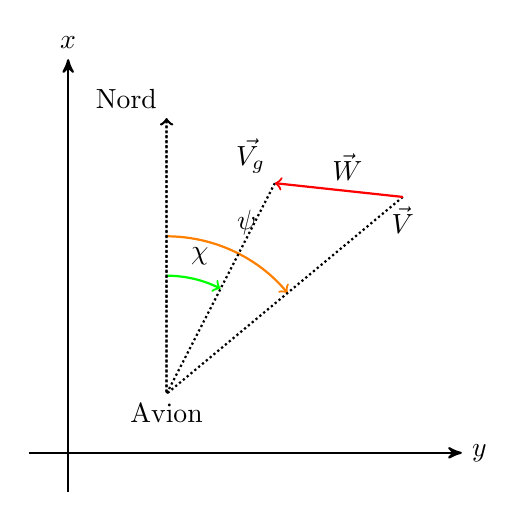
\begin{tikzpicture}[
        scale=5,
        axis/.style={thick, ->, >=stealth'},
        important line/.style={thick},
        dashed line/.style={dashed, thin},
        pile/.style={thick, ->, >=stealth', shorten <=2pt, shorten
        >=2pt},
        every node/.style={color=black}
        ]
        % axis
        \draw[axis] (-0.1,0)  -- (1, 0) node(xline)[right]{$y$};
        \draw[axis] (0, -0.1) -- (0, 1) node(yline)[above] {$x$};

        \coordinate (A) at (0.25, 0.15);
        \coordinate (N) at (0.25, 0.85);
        \coordinate (B) at (0.85, 0.65);
        \coordinate (C) at (0.525, 0.685)
        pic["$\psi$", draw=orange, <-, angle eccentricity=1.2, angle radius=2cm, important line]
        {angle=B--A--N}
        pic["$\chi$", draw=green, <-, angle eccentricity=1.2, angle radius=1.5cm, important line]
        {angle=C--A--N};

        \draw [densely dotted, thick, ->] (C)--(A)--(N);
        \draw [densely dotted, thick, ->] (B)--(A)--(N);

        \draw (A) node[below] {Avion};
        \draw (B) node[below] {$\vec{V}$};
        \draw (C) node[above left] {$\vec{V_g}$};
        \draw (N) node[above left] {Nord};
        \draw[important line, ->, draw=red] (B) --  (C)
            node[above right = -0.1 cm and 0.6 cm, text width=5em] {$\vec{W}$};

    \end{tikzpicture}
    \caption{Prise en compte du vent \( \vec{W} \)}\label{fig:M1}
    \end{center}
\end{figure}
\end{frame}

\begin{frame}
    \frametitle{Capture de route} \pause{}
    D'après la figure précedente, en notant
    \[ \underline{W} = {[W_x \quad W_y]}^T \quad \text{et}\quad \psi_w +
    \pi \quad \text{la direction du vent}\] \pause{}
    \[
    \underline{V}_g
    =
    \left[
    \begin{array}{c}
        V \cos (\gamma) \cos (\psi) + W \cos (\psi_w + \pi) \\
        V \cos (\gamma) \sin (\psi) + W \sin (\psi_w + \pi)
    \end{array}
    \right]
    =
    \left[
    \begin{array}{c}
        V_{g} \cos (\chi) \\
        V_{g} \sin (\chi)
    \end{array}
    \right]
    \] \pause{}
    D'où:
    \[
    \tan \chi = \frac
    {V \cos (\gamma) \sin (\psi) + W \sin (\psi_w + \pi)}
    {V \cos (\gamma) \cos (\psi) + W \cos (\psi_w + \pi)}
    \]
\end{frame}

\begin{frame}
    \frametitle{Capture de route} \pause{}
    En inversant l'équation précédente:
    \[
    \boxed{
    \psi_c=
    \chi_c + \arcsin
    \left(
    \frac
    {W_x \sin \chi_c - W_y \cos \chi_c}
    {V \cos \gamma}
    \right)
    }
    \]
\end{frame}

\begin{frame}
    \frametitle{Capture d'axe} \pause{}
    \begin{center}
        \begin{figure}

        \begin{tikzpicture}[scale=4.]
            % Axes
            \draw[->, thick] (0, 0) -- (1, 0) node [right] {$y$};
            \draw[->, thick] (0, 0) -- (0, 1) node [above] {$x$};

            % Points
            \coordinate (acft) at (.6, .3);
            \coordinate (btck) at (.1, .5);
            \coordinate (etck) at (0.35, .75);
            \coordinate (acftproj) at ($(btck)!(acft)!(etck)$);
            % Aircraft location
            \fill[red] (acft) circle (.5pt);
            \draw[dashed,red] (.6, 0.3) -- (.6, 0) node [below, red] {$y$};
            \draw[dashed,red] (.6, 0.3) -- (0, 0.3) node [left, red] {$x$};

            % Track
            \draw[->, green] (btck) -- (etck);
            \draw[dashed] (0.1, 0.8) -- (0.1, 0) node [below] {$y_a$};
            \draw[dashed] (0.1, 0.5) -- (0, 0.5) node [left] {$x_a$};
            \draw[->] (0.1, 0.7) arc (90:45:0.2) node [midway,above] {$\chi_a$};

            % Linking aircraft to track
            \draw[<->,blue] (acft) -- (acftproj) node[midway,right]{$e_y$};
            \draw[<->,blue] (btck) -- (acftproj) node[midway,right]{$e_x$};
        \end{tikzpicture}
        \caption{Vert: axe à capturer.
        Bleu: composantes \( \perp \) entre \( V \) et l'axe de piste. Rouge: avion}
    \end{figure}
    \end{center}
\end{frame}

\begin{frame}
    \frametitle{Capture d'axe} \pause{}
    Avec les notations précédentes:
    \[
    \left[
    \begin{array}{c}
        e_x \\
        e_y
    \end{array}
    \right]
    =
    \left[
    \begin{array}{cc}
        \cos \chi_a & \sin \chi_a \\
        - \sin \chi_a & \cos \chi_a
    \end{array}
    \right]
    \left[
    \begin{array}{c}
        x - x_a \\
        y - y_a
    \end{array}
    \right]
    \]
    En dérivant l'écart \( e_y \):
    \(
    \dot{e_y} = - \sin \chi_a \dot{x} + \cos \chi_a \dot{y}
    \)
    Avec:
    \[
    \left \{
    \begin{array}{l}
        \dot{x} = V_g \cos \chi \\
        \dot{y} = V_g \sin \chi
    \end{array}
    \right.
    \]
    On obtient:
    \[
    \dot{e_y} = V_g \sin (\chi_c - \chi_a)
    \]
\end{frame}

\begin{frame}
    \frametitle{Capture d'axe} \pause{}
    En considérant un retour du 1er ordre: (\( \dot{e_y} = -\frac{e_y}{\tau} \)):
    \pause{}
    \[
    \boxed{
        \chi_c = \chi_a - \arcsin (\frac{e_y}{\tau V_g})
    }
    \] \pause{}

    \[
    \left(
        \text{Pour l'implémentation:}
        \left \{
        \begin{array}{l}
            \dot{x} = V \cos (\gamma) \cos (\psi) + W_x \\
            \dot{y} = V \cos (\gamma) \sin (\psi) + W_y \\
        \end{array}
        \right.
    \right)
    \]
\end{frame}

\section{Conclusion}

\begin{frame}
    \frametitle{Conclusion} \pause{}

    \begin{center}
        À partir des équations simplifiées de la dynamique du point, et
        de commandes élémentaires (\( n_x \), \( n_z \) et \( p \)) on
        a réussi à mettre en place un système de commandes proche de
        la navigation d'un aéronef.
    \end{center}
\begin{center}
    Par la suite nous pourrions envisager de prendre en compte
    les performances de l'avion pour avoir une simulation plus
    en accord avec la réalité.

\end{center}

\end{frame}


\end{document}
